\documentclass[draft=True]{revtex4-2}
\documentclass[a4paper,10pt,draft]{thesis}
\usepackage{physics,amsmath, amsfonts, siunitx, amssymb, graphicx, slashed,subcaption}
\usepackage[utf8]{inputenc}
\usepackage[margin=1in]{geometry}
\usepackage[hidelinks]{hyperref}
\usepackage{xr-hyper}
\newcommand{\n}[1]{\nu_{#1}}
\newcommand{\na}{\nu_\alpha}
\newcommand{\nb}{\nu_\beta}
\newcommand{\ana}{\bar{\nu}_\alpha}
\newcommand{\an}[1]{\bar{\nu}_{\text{#1}}}
\newcommand{\anb}{\bar{\nu}_\beta}
\renewcommand{\a}{\alpha}
\renewcommand{\b}{\beta}
\newcommand{\ab}{\alpha\beta}


\renewcommand{\ne}{\nu_e}
\newcommand{\nm}{\nu_\mu}
\newcommand{\nt}{\nu_\tau}
\newcommand{\ns}{\nu_s}

\newcommand{\ane}{\bar{\nu}_e}
\newcommand{\anm}{\bar{\nu}_\mu}
\newcommand{\ant}{\bar{\nu}_\tau}
\newcommand{\ans}{\bar{\nu}_s}

\newcommand{\nee}{\nu_e \to \nu_e}
\newcommand{\nem}{\nu_e \to \nu_\mu}
\newcommand{\net}{\nu_e \to \nu_\tau}
\newcommand{\nes}{\nu_e \to \nu_s}

\newcommand{\nme}{\nu_\mu \to \nu_e}
\newcommand{\nmm}{\nu_\mu \to \nu_\mu}
\newcommand{\nmt}{\nu_\mu \to \nu_\tau}
\newcommand{\nms}{\nu_\mu \to \nu_s}



\newcommand{\Pee}{P_{e  e}}
\newcommand{\Pem}{P_{e  \mu}}
\newcommand{\Pet}{P_{e  \tau}}
\newcommand{\Pes}{P_{e  s}}

\newcommand{\Pme}{P_{\mu  e}}
\newcommand{\Pmm}{P_{\mu\mu}}
\newcommand{\Pmt}{P_{\mu  \tau}}
\newcommand{\Pms}{P_{\mu  s}}


\newcommand{\Pte}{P_{P_{\tau e}}}
\newcommand{\Ptm}{P_{\tau  \mu}}
\newcommand{\Ptt}{P_{\tau  \tau}}
\newcommand{\Pts}{P_{\mu  s}}

\newcommand{\Paeae}{P_{\bar{e}  \bar{e}}}
\newcommand{\Paeam}{P_{\bar{e}  \bar{\mu}}}
\newcommand{\Paeat}{P_{\bar{e}  \bar{\tau}}}
\newcommand{\Paeas}{P_{\bar{e}  \bar{s}}}

\newcommand{\Pamae}{P_{\bar{\mu}  \bar{e}}}
\newcommand{\Pamam}{P_{\bar{\mu}  \bar{\mu}}}
\newcommand{\Pamat}{P_{\bar{\mu}  \bar{\tau}}}
\newcommand{\Pamas}{P_{\bar{\mu}  \bar{s}}}


\newcommand{\Patae}{P_{\bar{\tau}  \bar{e}}}
\newcommand{\Patam}{P_{\bar{\tau}  \bar{\mu}}}
\newcommand{\Patat}{P_{\bar{\tau}  \bar{\tau}}}
\newcommand{\Patas}{P_{\bar{\mu}  \bar{s}}}

\renewcommand{\th}[1][]{%
  \theta\ifx\\#1\\\else_\text{#1}\fi
}
\newcommand{\thm}[1][]{%
  \theta^\text{M}\ifx\\#1\\\else_\text{#1}\fi
}
\renewcommand{\t}[1]{\text{{#1}}}
\newcommand{\avg}[1]{\left\langle {#1} \right \rangle}
\newcommand*{\dm}[1][]{%
  \Delta m^2\ifx\\#1\\\else_\text{#1}\fi
}
\newcommand{\zreco}{\cos{(\theta_z^{reco})}}
\newcommand{\ztrue}{\cos{(\theta_z^{true})}}
\newcommand{\z}{\cos{(\theta_z)}}
\newcommand{\Ereco}{E^{reco}}
\newcommand{\Etrue}{E^{true}}
\newcommand{\Aeff}{A^\text{eff}}
\newcommand{\emm}{\epsilon_{\mu\mu}}
\newcommand{\emt}{\epsilon_{\mu\tau}}
\newcommand{\eet}{\epsilon_{e\tau}}
\newcommand{\eem}{\epsilon_{e\mu}}
\newcommand{\ett}{\epsilon_{\tau\tau}}
\newcommand{\ep}{\epsilon^\prime}

\usepackage{physics,amsmath, amsfonts, siunitx, amssymb, graphicx, slashed}
\usepackage[utf8]{inputenc}
%\usepackage{hyperref}
\usepackage{xr-hyper}
\externaldocument{SM}

\begin{document}

\section{Neutrino Masses and Oscillations}\label{ch:oscillation}
As we saw in Eq.~\ref{eq:j_CC}
, the neutrino fields $\nu_\alpha$ only couple to the associated lepton fields $\ell_\alpha$, conserving the lepton number $L_\alpha$. We will now introduce two separate extensions to this part of the Standard Model.

We introduce a right-handed neutrino field, $\nu_R$. It has the usual properties of the conventional left-handed neutrino such as hypercharge and color zero. Moreover, since the electroweak gauge group $\t{SU}(2)_L$ only couple to left-handed particles and right-handed antiparticles, it transforms as a singlet under the SM symmetry group $\mathrm{SU}(3)_{\mathrm{C}} \times \mathrm{SU}(2)_{L} \times \mathrm{U}(1)_{Y}$. This neutrino is \emph{sterile} since it doesn't participate any of the SM interactions. 

We extend the SM by adding a right-handed component to the Higgs-lepton Yukawa Lagrangian from Eq.~\ref{eq:YukawaLagrangian} with neutrino Yukawa couplings $Y_{\alpha \beta}^{\prime \nu}$ ,

\begin{align}
    \mathcal{L}_{H}=-\left( \frac{v + H}{\sqrt{2}} \right) \left[\ell_{\alpha L}^{\prime} Y_{\alpha \beta}^{\prime \ell} \ell_{\beta R}^{\prime} + \nu_{\alpha L}^{\prime} Y_{\alpha \beta}^{\prime \nu} \nu_{\beta R}^{\prime}\right]
\end{align}
Similar to how we diagonalized the lepton Yukawa couplings $Y_{\alpha \beta}^{\prime \ell}$ in Eq.~~\ref{eq:leptonYukawaDiag}, we diagonalize $Y_{\alpha \beta}^{\prime \nu}$ as
\begin{align}
    V_{\alpha k L}^{\nu \dagger} Y^{\prime \nu}_{\alpha \beta} V_{\beta j R}^{\nu}=Y^{\nu}_{kj} \,.
\end{align}
Now we introduce a crucial difference between the properties of the charged lepton and the neutrino fields.
While the charged lepton flavor eigenstate was uniquely determined by its mass eigenstate, the neutrino flavor is a superposition of mass eigenstates. This is because neutrinos are indirectly detected via the observation of its associated charged lepton, so there is no requirement of neutrino flavor eigenstates to have a definite mass. The flavor of a neutrino is then, by definition, the flavor of the associated charged lepton. This is commonly introduced as giving the mass eigenstates Latin numerals and letters, while the flavor eigenstates stay as Greek letters.

So, let the neutrino field with chriality $X$ be denoted $\nu_X$, with components having Latin numerals to distinguish them from the flavour components, i.e 
\begin{align}\label{eq:nu_rotation}
    \nu_{k X} =  V_{k\beta X}^{\nu \dagger} \nu_{\beta X}^\prime\,.
\end{align}
The diagonalized Lagrangian now takes the form 
\begin{align}
    \mathcal{L}_{H} &= -\left( \frac{v + H}{\sqrt{2}} \right) \left[\ell_{\alpha L}^{\prime} Y_{\alpha \beta}^{\prime \ell} \ell_{\beta R}^{\prime} + \nu_{\alpha L}^{\prime} Y_{\alpha \beta}^{\prime \nu} \nu_{\beta R}^{\prime}\right] \nonumber \\
    &= -\left( \frac{v + H}{\sqrt{2}} \right) \left[\ell_{\alpha L}^{\prime} V_{\alpha \beta L}^{\ell} Y_{\alpha \beta}^{ \ell} V_{\alpha \beta R}^{\ell \dagger} \ell_{\beta R}^{\prime}\right. \nonumber \\
    &\hspace{5.7em}+\left. \nu_{\alpha L}^{\prime} V_{\alpha k L}^{\nu} Y_{kj}^{\nu} V_{\beta j  R}^{\nu \dagger} \nu_{\beta R}^{\prime}\right] \nonumber \\
    &= -\left( \frac{v + H}{\sqrt{2}} \right) \left[\ell_{\alpha L}^\dagger Y_{\alpha \beta}^{ \ell} \ell_{\beta R} + \nu_{k L}^{\dagger} Y_{kj}^{ \nu} \nu_{j R}\right] \nonumber \\
    &= -\left( \frac{v + H}{\sqrt{2}} \right) \left[\bar{\ell}_{\alpha L} Y_{\alpha \beta}^{ \ell} \ell_{\beta R} + \bar{\nu}_{k L} Y_{kj}^\nu \nu_{j R}\right]
\end{align}
By construction, $Y^\ell_{\alpha \beta}$ and $Y^\nu_{kj}$ are diagonal, so we write them as $y_{\alpha}^{\ell} \delta_{\alpha \beta}$ and $y_{k}^{\nu} \delta_{k j}$ respectively, leaving the Lagrangian as 
\begin{align}\label{eq:L_H}
    \mathcal{L}_{H} 
    &=-\left( \frac{v + H}{\sqrt{2}} \right) \left[\bar{\ell}_{\alpha L} y_{\alpha}^{\ell} \delta_{\alpha \beta} \ell_{\beta R} + \bar{\nu}_{k L} y_{k}^{\nu} \delta_{k j} \nu_{j R}\right] \nonumber \\
    &=-\left( \frac{v + H}{\sqrt{2}} \right) \left[\bar{\ell}_{\alpha L} y_{\alpha}^{\ell}  \ell_{\alpha R} + \bar{\nu}_{k L} y_{k}^{\nu} \nu_{k R}\right] \nonumber \\
    &=-\left( \frac{v + H}{\sqrt{2}} \right) \left[ y_{\alpha}^{\ell}  \bar{\ell}_{\alpha L}\ell_{\alpha R} +  y_{k}^{\nu}\bar{\nu}_{k L} \nu_{k R}\right] 
\end{align}

Now, the Dirac neutrino field is
\begin{align}
    \nu_k = \nu_{kL} + \nu_{kR}\,.
\end{align}
Multiplying $\nu_k$ with its conjugate $\bar{\nu}_k$, we get 
\begin{align}
    \bar{\nu}_k \nu_k 
    & = \bar{\nu}_{k L} \nu_{k L} +\bar{\nu}_{k R}\nu_{k L} + \bar{\nu}_{k L}\nu_{k R} + \bar{\nu}_{k R}\nu_{k R} \nonumber \\
    & = \bar{\nu}_{k L}\nu_{k R} + \bar{\nu}_{k R}\nu_{k L} \nonumber \\
    & = \bar{\nu}_{k L}\nu_{k R} + \t{h.c.}
\end{align}
The same calculation for the charged lepton field yields the same result for $\ell_k$. Substituting this result and expanding the Higgs VEV into the fields gives us
\begin{align}
    \mathcal{L}_{H} 
    &=-\left( \frac{v + H}{\sqrt{2}} \right) \left[ y_{\alpha}^{\ell}   \bar{\ell}_\alpha \ell_\alpha  +  y_{k}^{\nu} \bar{\nu}_k \nu_k \right] \nonumber \\
    &=- \frac{y_{\alpha}^{\ell} v}{\sqrt{2}}   \bar{\ell}_\alpha \ell_\alpha   -  \frac{ y_{k}^{\nu} v}{\sqrt{2}} \bar{\nu}_k \nu_k  - \frac{y_{\alpha}^{\ell}}{\sqrt{2}}   \bar{\ell}_\alpha \ell_\alpha H  -  \frac{ y_{k}^{\nu}}{\sqrt{2}} \bar{\nu}_k \nu_k H\,.
\end{align}
Thus, this extension to the SM generates neutrino masses by the Higgs mechanism, in the same fashion as with the charged leptons and the quarks:
\begin{align}
    m_k = \frac{y_k^\nu v}{\sqrt{2}}
\end{align}

Substituting the new transformation from Eq.~\ref{eq:nu_rotation} into the weak charged current, we get
\begin{align}\label{eq:j_CC2}
    j^\rho_L &= 2\bar{\nu}^\prime_{\alpha L} \gamma^\rho \ell_{\alpha L}^\prime \nonumber \\
             &= 2\bar{\nu}_{k L} V^{\prime \nu \dagger}_{k \alpha}V^{\prime \ell}_{\alpha \alpha} \gamma^\rho  \ell_{\alpha L}
\end{align}
Call $V^{\prime \nu \dagger}_{k \alpha}V^{\prime \ell}_{\alpha \alpha} = U^\dagger_{k \alpha}$
Now, the current in Eq.~\ref{eq:j_CC2} conserves lepton number, since the neutrino field with flavor $\alpha$ only couples to the lepton field with flavor $\alpha$. However, the Higgs-lepton Yukawa Lagrangian 
in Eq.~\ref{eq:L_H} violates lepton number conservation since it couples the charged lepton flavor $\alpha$ to the neutrino mass eigenstate $k$, which is a superposition of flavors. There is no transformation that leaves both the interaction and kinetic Lagrangian invariant.
We now have 
\begin{align}\label{eq:j_CC3} %TODO: put sums on all above?
    j^\rho_L &= 2 \sum_\alpha \sum_k U^*_{\alpha k} \bar{\nu}_{k L} \gamma^\rho  \ell_{\alpha L}
\end{align}
Now, the Fourier expansion of the field operator $\bar{\nu}_{k L}$ in Eq.~\ref{eq:j_CC3} contains creation operators $a^\dagger_{\nu_k}$
of massive neutrinos with mass $m_k$. This means that the summation over the mass index $k$ constructs a flavor neutrino, which interacts with the charged lepton field $\ell_{\a L}$.
In other words, the charged current generates a flavor neutrino $\na$, which is a superposition of the mass eigenstates 
$\nu_k$ with weights $U_{\a k}^*$. In the ket-formalism, we express this as
\begin{align}\label{eq:osc_1}
    \ket{\na} = \sum_k U^*_{\a k} \ket{\nu_k}\,.
\end{align}
It is the mass eigenstates $\ket{\nu_k}$ that are eigenstates of the Hamiltonian, with eigenvalues
\begin{align}\label{eq:disp}
    E_k = \sqrt{\vec{p}^2 + m_k^2}\,.
\end{align}
The solution to the time-dependent Schrödinger equation 
\begin{align}\label{eq:TDSE}
    i \dv{}{t} \ket{\nu_k(t)} = H_0\ket{\nu_k(t)}\,,
\end{align}
where $H_0$ is the Hamiltonian and the subscript signifies that we are in vacuum. 

The solution to Eq.~\ref{eq:TDSE} gives ut the time evolution
in the form of plane wave solutions: 
\begin{align}
    \ket{\nu_k(t)} = e^{-iE_kt}\ket{\nu_k}\,.
\end{align}
Inserting the plane wave solution into Eq.~\ref{eq:osc_1}, we get 
\begin{align}\label{eq:nat}
    \ket{\na(t)} = \sum_k U^*_{\a k} e^{-iE_kt}\ket{\nu_k}\,.
\end{align}
Now we know how to evolve and combine the mass eigenstates to form a flavor eigenstate, but how about the reverse? We swap the index $k\to j$ in Eq.~\ref{eq:osc_1} and multiply by $U_{\a k}$:
\begin{align}\label{eq:osc_k}
    \sum_\a U_{\a k}\ket{\na} &= \sum_{\alpha, j} U_{\a k} U_{\a j}^* \ket{\nu_j} \nonumber \\
    \sum_\a U_{\a k}\ket{\na} &= \sum_{j} \delta_{kj} \ket{\nu_j} \nonumber \\
    \sum_\a U_{\a k}\ket{\na} &= \ket{\nu_k}\,,
\end{align}
where we have used the unitarity of the leptonic mixing matrix. Eqs.~\ref{eq:osc_1} and \ref{eq:nat} yield 
\begin{align}
    \ket{\na(t)} &= \sum_k U^*_{\a k} e^{-iE_kt}\ket{\nu_k} \nonumber \\
    \ket{\na(t)} &= \sum_k U^*_{\a k} e^{-iE_kt}\left(\sum_\b U_{\b k}\ket{\nb}\right) \nonumber \\
    \ket{\na(t)} &= \sum_{k,\b} U^*_{\a k}U_{\b k} e^{-iE_kt} \ket{\nb}\,.
\end{align}
The probability of the flavor transition $\na \to \nb$ at time $t$ is $\abs{\bra{\nb}\ket{\na (t)}}^2$:
\begin{align}
    P_{\na \to \nb}(t) = \sum_{k,j} U^*_{\a k}U_{\b k}U^*_{\b j}U_{\a j} e^{-i(E_k-E_j)t}\,.
\end{align}

We assume the neutrino masses $m_k$ to be extremely small compared to their associated energies $E_k$. Thus, $v\approx 1$, and $\abs{\vec{p}} \approx E$ making the energy-dispersion relation of Eq.~\ref{eq:disp} to first order:
\begin{align}\label{eq:ultra_rel}
    E_k &= \sqrt{\vec{p}^2 + m_k^2} \nonumber \\
        &= \vec{p}^2\sqrt{1 + \frac{m_k^2}{\vec{p}^2}} \nonumber \\
        &\approx E + \frac{m_k^2}{2E}
\end{align}
Hence, the exponential can be simplified, and simplifying the notation $P_{\na \to \nb}(t) \to P_{\ab}(t)$ we get 
\begin{align}
    P_{\ab}(t) = \sum_{k,j} U^*_{\a k}U_{\b k}U^*_{\b j}U_{\a j} e^{-i(m_k^2-m_j^2)t/2E}\,.
\end{align}

Now, our approximation $v\approx 1$ implies $x\approx t $, thus
\begin{align}
    P_{\ab}(x) &= \sum_{k,j} U^*_{\a k}U_{\b k}U^*_{\b j}U_{\a j} e^{-i(m_k^2-m_j^2)x/2E} \nonumber \\
                       &= \sum_{k,j} U^*_{\a k}U_{\b k}U^*_{\b j}U_{\a j} \exp(-i\frac{\dm_{kj}x}{2E})\,,
\end{align}
where we in the last step have defined the \emph{mass squared-difference} $\dm_{kj} = m_k^2 - m_j^2$. Since the oscillation probability depends on this quantity
rather than the individual masses, it is impossible
to measure the mass states $m_k$ through neutrino oscillations.
Squaring the unitarity condition $\sum_k U_{\a k}U_{\b k}^* = \delta_{\a \b}$ yields 
\begin{align}
    \sum_k \abs{U_{\a k}}^2\abs{U_{\b k}}^2 = \delta_{\a \b} - 2 \sum_{k>j}\Re[U_{\a k}^* U_{\b k} U_{\a j} U_{\b j}^*]
\end{align}
In this work, we will always assume the mixing matrix $U$ to be real. 
We thus write 
\begin{align}\label{eq:Pab}
    P_{\ab} &= \sum_{k,j} U_{\a k}U_{\b k}U_{\b j}U_{\a j} \exp(-i\frac{\dm_{kj}x}{2E}) \nonumber \\
            &=  \sum_k \abs{U_{\a k}}^2\abs{U_{\b k}}^2 + \nonumber \\
            &\hspace{2em}+ \sum_{k \neq j} U_{\a k}U_{\b k}U_{\b j}U_{\a j} \exp(-i\frac{\dm_{kj}x}{2E}) \nonumber \\
            &= \delta_{\a \b} - 2 \sum_{k>j}U_{\a k} U_{\b k} U_{\b j} U_{\a j} \nonumber \\
            & \hspace{3em}+\sum_{k \neq j} U_{\a k}U_{\b k}U_{\b j}U_{\a j} \exp(-i\frac{\dm_{kj}x}{2E}) \nonumber \\
            &= \delta_{\a \b} - 2 \sum_{k>j}U_{\a k} U_{\b k} U_{\b j} U_{\a j} \nonumber \\
            &\hspace{3em}+ 2\sum_{k > j} U_{\a k}U_{\b k}U_{\b j}U_{\a j} \exp(-i\frac{\dm_{kj}x}{2E}) \nonumber \\
            &= \delta_{\a \b} - 2\sum_{k > j} U_{\a k}U_{\b k}U_{\b j}U_{\a j} \left[1-\exp(-i\frac{\dm_{kj}x}{2E})\right] \nonumber \\
            &= \delta_{\a \b} - 2\sum_{k > j} U_{\a k}U_{\b k}U_{\b j}U_{\a j} \left[1-\cos(\frac{\dm_{kj}x}{2E})\right] \nonumber \\
            &= \delta_{\a \b} - 2\sum_{k > j} U_{\a k}U_{\b k}U_{\b j}U_{\a j} \sin^2{\left(\frac{\dm_{kj}x}{4E}\right)}\,,
\end{align}
which is the probability of neutrino vacuum oscillations. %TODO: maybe plot?
The calculation for antineutrinos yield the same result if one assumes the realness of the mixing matrix. 

\subsection{Matter effects}
\begin{figure}\label{fig:w_and_z}
    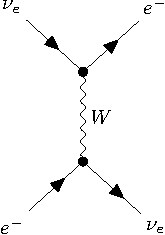
\includegraphics[width=0.1\textwidth]{figures/w-boson.pdf}
    \hspace{2cm}
    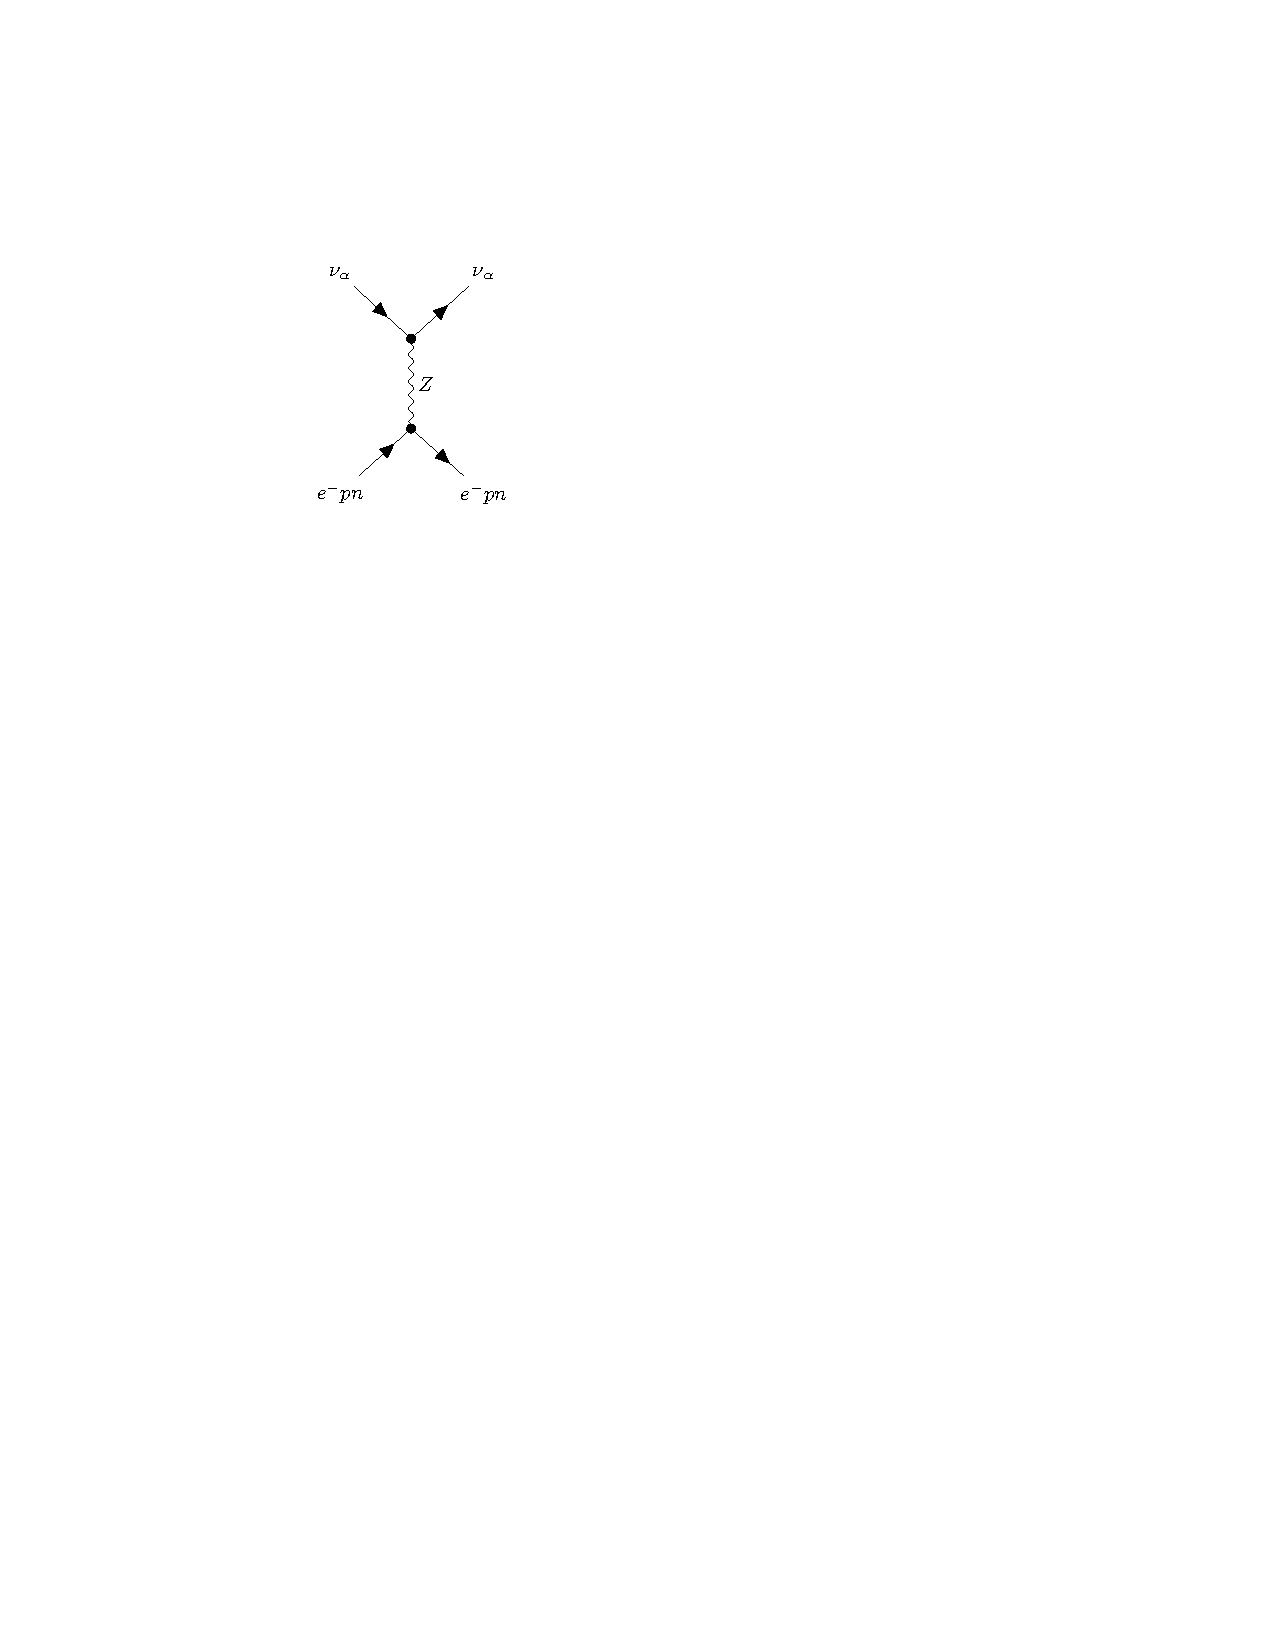
\includegraphics[width=0.1\textwidth]{figures/z-boson.pdf}
\end{figure}
In this work, we are concerned about the interactions with the neutrino and Earth-like matter, i.e. electrons, protons, and neutrons. 
The possible interactions are shown in Fig. ~\ref{fig:w_and_z}. The left panel shows that the only flavor that can go through charged current (CC) 
interactions is the electron flavor. This is because the Earth doesn't consist of any muons or tau particles. 
The right panel shows any neutrino flavor interaction via the neutral current (NC) with Earth-like matter, mediated by the neutral $Z$ boson
 we see weak forward CC and NC scattering. 
The interaction mediated by the $W$ boson will give rise to a effective matter potential $V_{CC}$, while
the $Z$ boson is responsible for $V_{NC}$. Our task is now to find expressions for these.

\subsection{Effective matter potentials}

We start with the effective Hamiltonian for the CC process. The Feynman rules for the left panel give us 
\begin{align}
    H^{CC} = \frac{G_F}{\sqrt{2}}\left[ \bar\ne \gamma^\rho\, (1- \gamma^5)\, e \right] \left[\bar e \,\gamma_\rho\, (1- \gamma^5)\, \ne \right]
\end{align}
By using the Fierz transformation 
\begin{align}
    \mathcal{L}^{V-A}(\psi_1,\psi_2,\psi_3,\psi_4) = \mathcal{L}^{V-A}(\psi_1,\psi_4,\psi_3,\psi_2)\,,
\end{align}
we can permute the terms inside the brackets, yielding
\begin{align}\label{eq:H_fierz}
    H^{CC} = \frac{G_F}{\sqrt{2}}\left[ \bar\ne \gamma^\rho\, (1- \gamma^5)\, \ne \right] \left[\bar e \,\gamma_\rho\, (1- \gamma^5)\, e \right]\,.
\end{align}
Now, lets consider a finite volume $V$ with electron states defined as 
\begin{align}\label{eq:e_states}
    \ket{e(p_e,h_e)} = \frac{1}{2E_eV}a_e^{(h_e)\dagger}(p_e)\ket{0}\,,
\end{align}
i.e. using the creation operator $a_e^{(h_e)\dagger}(p_e)$ to create electron states from vacuum with momenta $p_e$, energy $E_e$, and helicity $h_e$.
The density distribution of electrons in $V$ is $f(E_e,T)$, which we normalize to the total number of electrons as we integrate out the momenta $p_e$:
\begin{align}\label{eq:e_density}
    \int \dd p_e^3 f(E_e,T) = N_e V = n_e
\end{align}
Here, the electron density $N_e$ will ultimately determine the strength of the effective matter potential. 
To obtain the average effective Hamiltonian, project it on the electron states in Eq.~\ref{eq:e_states} and integrate over the density and sum over the helicities:

\begin{align}\label{eq:avg_H1}
    \bar{H}^{CC} &= \int \dd p_e^3 \bra{e(p_e,h_e)} \times \frac{1}{2} \sum_{h_e} H   f(E_e,T) \ket{e(p_e,h_e)} \nonumber \\
           &= \frac{G_F}{\sqrt{2}} \int \dd p_e^3 \bra{e(p_e,h_e)} \left[ \bar\ne \gamma^\rho\, (1- \gamma^5)\, \ne \right]  f(E_e,T) \times \frac{1}{2} \sum_{h_e} \left[\bar e(x) \,\gamma_\rho\, (1- \gamma^5)\, e(x) \right] \ket{e(p_e,h_e)} \nonumber \\
           &= \frac{G_F}{\sqrt{2}} \bar\ne \gamma^\rho\, (1- \gamma^5)\, \ne \int \dd p_e^3  f(E_e,T) \times \frac{1}{2} \sum_{h_e} \bra{e(p_e,h_e)} \bar e(x) \,\gamma_\rho\, (1- \gamma^5)\, e(x)   \ket{e(p_e,h_e)}\,.
\end{align}
First, calculate the sum using trace technology %TODO: explain this more
\begin{align}\label{eq:helicity_sum}
    \frac{1}{2} \sum_{h_e} \bra{e(p_e,h_e)} \bar e(x) \,\gamma_\rho\, (1- \gamma^5)\, e(x)   \ket{e(p_e,h_e)} &= \frac{1}{4E_e V} \sum_{h_e} \bar{u}_e^{h_e}(p_e) \,\gamma_\rho\, (1- \gamma^5)\, u_e^{h_e}(p_e) \nonumber \\
    &= \frac{1}{4 E_e V} \Trace{\left[ \sum_{h_e} \bar{u}_e^{h_e}(p_e) u_e^{h_e}(p_e) \,\gamma_\rho\, (1- \gamma^5)\, \right]} \nonumber \\
    &= \frac{1}{4 E_e V} \Trace{\left[ (\slashed{p}_e + m_e ) \,\gamma_\rho\, (1- \gamma^5)\, \right]} \nonumber \\
    &= \frac{(p_e)_\rho}{E_e V}\,.
\end{align}
Eq.~\ref{eq:avg_H1} now becomes 
\begin{align}\label{eq:avg_H2}
    \avg{H^{CC}} &= \frac{G_F}{\sqrt{2}E_e V} \bar\ne \, (1- \gamma^5)\, \ne \int \dd p_e^3\, \slashed{p}_e\, f(E_e,T)\,.
\end{align}
Expand the integral, and use the fact that $\vec{p}_e$ is odd:
\begin{align}
    \int \dd p_e^3\, \slashed{p}_e\, f(E_e,T) &= \int \dd p_e^3\, f(E_e,T) (\gamma^0 E_e - \vec{p}_e \cdot \vec{gamma}) \nonumber \\
                                              &= \int \dd p_e^3\, f(E_e,T) \gamma^0 E_e \nonumber \\
                                              &= \gamma_0 E_e N_e V\,.
\end{align}
Inserting this into Eq.~\ref{eq:avg_H2}, we have
\begin{align}
    \avg{H^{CC}} &= \frac{G_F N_e}{\sqrt{2}} \bar{\nu}_e \, (1- \gamma^5)\, \ne \gamma_0 \nonumber \\
            &= \sqrt{2}G_F N_e \bar{\nu}_{Le} \gamma^0 \nu_{Le}\,,
\end{align}
where the projection operator $(1- \gamma^5)$ ensures that only the left-hand compontent of the neutrino fields interact weakly. Thus,
\begin{align}\label{eq:V_CC1}
    V_{CC} = \sqrt{2}G_F N_e\,, \quad H^{CC}\ket{\nu_k} = V_{CC}\ket{\nu_k}\,.
\end{align}
Here we see a crucial difference between the eigenvectors between the vacuum Hamiltonian defined in Eq.~\ref{eq:osc_1} and $H^{CC}$, namely
that the CC (and NC) interactions happen in the flavor basis rather than in the mass basis. In other words,
neutrinos propagate in their mass eigenstates, but interact in their flavor eigenstate. The mixing of mass eigenstates during propagation
determines if the flavor eigenstate has oscillated or not. Thus, the expressions involving the 
matter potential does not need to be transformed by the PMNS matrix.

For neutral current, we replace the electron field $e(x)$ in Eq.~\ref{eq:H_fierz} by the fermion field $f(x)$, and the projection operator 
$(1-\gamma^5)$ with $(g_V^f - g_A^f\gamma^5)$. Again, the $\gamma^5$ will cause the spacial component of $p_f$ to disappear after integration, and the 
only difference between the average effective Hamiltonian for the neutral current is then the factor $g_V^f$:
\begin{align}
    V^f_{NC} = \sqrt{2}G_F N_A g_V^f\,.
\end{align}
Summing over the fermions, and assuming electrical neutrality and equal abundance of protons and neutrons, we have
\begin{align}
    V_{NC} &= \sum_{f \in {e,p,n}} V^f_{NC} \nonumber \\
           &= \sqrt{2}G_F N_A \sum_{f \in {e,p,n}} g_V^f \nonumber \\
           &= \sqrt{2}G_F N_A\left[ -\frac{1}{2}+2\sin^2{(\theta_W)} + \frac{1}{2}-2\sin^2{(\theta_W)} -\frac{1}{2} \right] \nonumber \\
           &= -\frac{1}  {\sqrt{2}} G_F N_e\,,
\end{align}
where the electrical neutrality condition allows us to simply sum the vectorial couplings together, cancelling the electron and proton contributions (and hence, also the mixing angle dependence).
\subsection{Matter oscillations}
Since only $\ne$ undergo CC interactions in Earth-like matter, the $V_{CC}$ potential is zero for all other flavors. However, since all flavors undergo NC interactions the total matter potential in matrix form is:
\begin{align}\label{V_matrix}
    V = \begin{bmatrix}
        V_{CC} + V_{NC} & 0 & 0 \\
        0 & V_{NC} & 0 \\
        0 & 0 & V_{NC} \\
    \end{bmatrix} = V_{CC}\, \delta_{\alpha e} + V_{NC}\,.
\end{align}

Just as in Eq.~\ref{eq:TDSE}, we start with a Hamiltonian that solves the time-dependent Schrödinger equation. This time, let the Hamiltonian be 
\begin{align}
    H = H_0 + H_{I}\,,
\end{align}
where $H_0$ is the Hamiltonian in vacuum, and $H_{I}$ is our interaction Hamiltonian associated with our matter potentials.
Let the wavefunction that describes the $\nu_\a \to \nu_\b$ transition be 
\begin{align}
    \bra{\nu_\b}\ket{\nu_\a (t)}\,,
\end{align}
i.e.~the evolution of the state of a neutrino emitted at $t =0$ with flavor $\alpha$ to flavor $\beta$ at time $t$.

Now using Eq.~\ref{eq:osc_1} and Eq.~\ref{eq:V_CC1}, we are ready to see what form our Hamiltonians take.
Let us start with the vaccum Hamiltonian $H_0$, and act on its Schrödinger equation with $\bra{\nu_\b}\,$:
\begin{align}
    i \dv{}{t}\ket{\nu_\a (t)} = H_0\ket{\nu_\a (t)} \implies i \dv{}{t}\psi_{\a\b} = \bra{\nu_\b}H_0\ket{\nu_\a (t)}\,.
\end{align}
Reminding ourselves that the vacuum Hamiltonian $H_0$ has eigenstates in the mass basis, we write the following expression where 
use the relations ~\ref{eq:osc_1} and ~\ref{eq:osc_k} to switch between the flavor and mass basis with the PMNS elements:
\begin{align}
    \bra{\nu_\b} H_0 &= \sum_k U_{\b k} \bra{\nu_k}H_0 \nonumber \\
                     &= \sum_k U_{\b k} E_k \bra{\nu_k} \nonumber \\
                     &= \sum_\eta \sum_k U_{\b k} E_k U^*_{\eta k} \bra{\nu_\eta}\,.
\end{align}
Thus,
\begin{align}
    \bra{\nu_\b}H_0\ket{\nu_\a (t)} &= \sum_\eta \sum_k U_{\b k} E_k U^*_{\eta k} \bra{\nu_\eta}\ket{\nu_\a (t)} \nonumber \\
                                    &= \sum_\eta \sum_k U_{\b k} E_k U^*_{\eta k} \psi_{\a\eta}(t)\,.
\end{align}
Using the ultrarelativistic approximation from Eq.~\ref{eq:ultra_rel}:
\begin{align}
    \sum_\eta \sum_k U_{\b k} E_k U^*_{\eta k} \psi_{\a\eta}(t) &= \sum_\eta \sum_k U_{\b k} \left(p + \frac{m^2_k}{2E}\right) U^*_{\eta k} \psi_{\a\eta}(x) \nonumber \\
    &= \sum_\eta \sum_k U_{\b k} \left(p + \frac{m^2_k}{2E}\right) U^*_{\eta k} \psi_{\a\eta}(x)\,.
\end{align}
Use the fact that $\sum_k m_k^2 = \sum_k m_1^2 + m^2_k - m^2_1 = m_1^2 + \sum_k \dm_{k1}$ to pull out common terms out of the summation:
\begin{align}\label{eq:t1}
    \sum_\eta \sum_k U_{\b k} \left(p + \frac{m^2_k}{2E}\right) U^*_{\eta k} \psi_{\a\eta}(x) &= \sum_\eta \sum_k U_{\b k} \left(p + \frac{m^2_1}{2E} + \frac{\dm_{k1}}{2E}\right) U^*_{\eta k} \psi_{\a\eta}(x) \nonumber \\
    &= \sum_\eta\sum_k \left(p + \frac{m^2_1}{2E}\right) U_{\b k} U^*_{\eta k} \psi_{\a\eta}(x) + \sum_\eta\sum_k U_{\b k} \frac{\dm_{k1}}{2E} U^*_{\eta k} \psi_{\a\eta}(x)\,.
\end{align}
Unitarity gives $ \sum_k U_{\b k} U^*_{\eta k} = \delta_{\eta\b}$, and the first term in the last step of Eq.~\ref{t1} becomes
\begin{align}
    \sum_\eta \left(p + \frac{m^2_1}{2E}\right) \delta_{\beta \eta} \psi_{\a\eta}(x)
    =& \left(p + \frac{m^2_1}{2E}\right) \psi_{\a\b}(x)\,.
\end{align}
This is a phase common to all states, which does not affect the probability since it can be rotated away.
Our treatment of the interaction Hamiltonian is similar except for the fact that its eigenstates lie in the flavor basis, conviniently allowing us
to letting it act directly on the flavor eigenstates:
\begin{align}
    \bra{\nu_\b}H_I &= V_\beta \bra{\nu_\b} \nonumber\\
                    &= \delta_{\b\eta} V_\beta \bra{\nu_\eta}\,.
\end{align}  
%\bibliographystyle{apalike}
%\bibliography{ref}
\end{document}